\documentclass[a4paper]{article}
\usepackage[utf8]{inputenc}
\usepackage[english]{babel}
\usepackage{listings}
\usepackage{xcolor}
\usepackage[braket, qm]{qcircuit} % Importa il pacchetto qcircuit
\lstdefinestyle{python}{
    language=Python,
    basicstyle=\ttfamily\small,
    keywordstyle=\color{blue},
    stringstyle=\color{red},
    commentstyle=\color{green},
    morecomment=[s][\color{purple}]{/**}{*/},
    numberstyle=\tiny\color{gray},
    stepnumber=1,
    numbersep=10pt,
    frame=single,
    breaklines=true,
    postbreak=\mbox{\textcolor{red}{$\hookrightarrow$}\space},
    showspaces=false,
    showstringspaces=false
}
\lstset{style=python}

%\newtheorem{theorem}{Theorem}
\usepackage{amsmath, amssymb, graphicx, algorithm, algpseudocode}

\linespread{1.7}
%\usepackage{fullpage}
\title{Genetic algorithm for Quantum Support Vector Machines}
\author{Lorenzo Tasca}
\date{October 2024}

\begin{document}

%\setlength{\parindent}{0pt}
\maketitle
\tableofcontents

\newpage


\section{Introduction}


\section{Classical machine learning}

\subsection{General overview}
baa
\subsection{Support vector machine}



The Support Vector Machine (SVM) is a binary classification algorithm, whose goal is to build the maximum margin separator between the two classes, that is the separator that maximizes the distance of the closest point from each class. The standard SVM algorithm is a linear algorithm, so in particular it will try and build the separating margin as a hyperplane in a $d$-dimensional space (so a $(d-1)$-dimensional plane), where $d$ is the number of features. The points that touch the margin, or that are on the wrong side of it, are called support vectors. The distance between the decision boundary and the support vectors is called margin. The algorithm will find the biggest possible margin. 

\subsubsection{Linear SVM}
Let's start assuming that the classes are linearly separable. We are provided with a dataset with $N$ $d$-dimensional instances $\{\mathbf{x}_i\}_{i=0,\cdots, N-1}$. The two classes will be labelled with $$y\in \{-1,1\}.$$ The margin will be the set of points 
\begin{equation}
    \{\mathbf{x}\in\mathbb{R}^d: w_0+\mathbf{w}^T\cdot \mathbf{x}=0\},
    \label{margin definition}
\end{equation}  
for appropriate parameters $w_0\in \mathbb{R}$ and $\mathbf{w}\in \mathbb{R}^d$, which define the hyperplane and must be found by the algorithm. Now we have to find $$\max_{w_0, \mathbf{w}}(m),$$ with the constraint 
\begin{equation}
    \frac{1}{||\mathbf{w}||}y_i(w_0+\mathbf{w}^T\cdot \mathbf{x_i})\geq m, \, \forall i=0,\cdots, N-1,
\end{equation}
that can be rewritten as 
\begin{equation}
    y_i(w_0+\mathbf{w}^T\cdot \mathbf{x_i})\geq m||\mathbf{w}||, \, \forall i=0,\cdots, N-1.
\end{equation}
The constraint prevents data points from falling into the margin. Rescaling $\mathbf{w}$ up to a multiplicative factor does not change the hyperplane it defines, so for convenience we can choose its norm such that 
\begin{equation}
    ||\mathbf{w}||=\frac{1}{m}.
\end{equation}
Therefore, the problem becomes minimizing
$$\frac{1}{2}||\mathbf{w}||, $$ with the constraint 
\begin{equation}
    y_i(w_0+\mathbf{w}^T\cdot \mathbf{x_i})\geq 1, \, \forall i=0,\cdots, N-1.
    \label{constraint hard margin}
\end{equation}
In the theory of convex optimization one can solve for the Lagrangian dual of this problem. We can introduce the dual variables $\alpha_i$ such that
\begin{equation}
    \mathbf{w}=\sum_{i=0}^{N-1}\alpha_iy_i\mathbf{x}_i.
    \label{alpha def}
\end{equation} 
One would obtain that the dual problem consists in maximizing, with respect to the weight vector $\mathbf{\alpha}\in\mathbb{R}^N$, the expression 
\begin{equation}
    f(\alpha_0,\cdots,\alpha_{N-1})=\sum_{i=0}^{N-1} \alpha_i-\frac{1}{2}\sum_{i=0}^{N-1}\sum_{j=0}^{N-1}\alpha_i\alpha_jy_iy_j(\mathbf{x}_i,\mathbf{x}_j),
    \label{dual problem SVM}
\end{equation}
with the constraint
\begin{equation}
    \alpha_i\geq 0,\,\forall i=0,\cdots, N-1,
\end{equation}
\begin{equation}
    \sum_{i=0}^{N-1}\alpha_iy_i=0.
\end{equation}
In eq. (\ref{dual problem SVM}) we indicated as $(\mathbf{x}_i,\mathbf{x}_j)$ the standard dot product of $\mathbb{R}^d$, explicitly
$$(\mathbf{x}_i,\mathbf{x}_j)=\mathbf{x}_i^T\cdot\mathbf{x}_j=\sum_{k=0}^{d-1}(\mathbf{x}_i)_k(\mathbf{x}_j)_k.$$
Eq. (\ref{dual problem SVM}) defines a quadratic programming
optimization problem, therefore the global maximum of $f$ can be efficiently found in the context of convex analysis. The parameter $w_0$ can be found by imposing that, for a support vector $$y_i(\mathbf{w}^T\mathbf{x}_i+w_0)=1,$$ that is 
\begin{equation}
    w_0=\mathbf{w}^T\mathbf{x}_i-y_i.
\end{equation} 
Once the optimal $\alpha_i$ have been found, given a new instance $\mathbf{\tilde{x}}$, according to eq. (\ref{alpha def}) and eq. (\ref{margin definition}), we can predict its class calculating 
\begin{equation}
    \textup{sign}\left[\sum_{i=0}^{N-1}\alpha_iy_i(\mathbf{\tilde{x}}, \mathbf{x}_i)+w_0\right].
    \label{decision boundary svm}
\end{equation} 

What we just described is the so-called hard margin SVM, because we did not allow points to fall inside the margin. One could relax this assumption, modifying the constraint in eq. (\ref{constraint hard margin}) into 
\begin{equation}
    y_i(w_0+\mathbf{w}^T\cdot \mathbf{x_i})\geq 1-\xi_i, \, \forall i=0,\cdots, N-1,
\end{equation}
where we introduced the slack variables $\xi_i$. We limit the softness of the margin by setting a positive constant $C$ such that 
$$ \xi\geq0,$$
\begin{equation}
    \sum_{i=0}^{N-1}\xi_i\leq C.
\end{equation}
This is called soft margin SVM. 

scikit-learn provides a straightforward implementation of the SVM algorithm, which we can use to observe the algorithm in action through an example. We use a mock dataset with 2 features, so we can easily print the data, the decision boundary and the margin. 


\begin{lstlisting}
from sklearn.svm import SVC
from sklearn.datasets import make_blobs 

X,y = make_blobs(n_samples=200) #create mock dataset
svm = SVC(kernel='linear', C=1) #create svm
svm.fit(X, y) #fit the svm
\end{lstlisting}

The result of the fit is shown in Figure (\ref{fig:classical svm mock}). We can observe how the algorithm built the largest possible margin. 


\begin{figure}[h!]
    \centering
    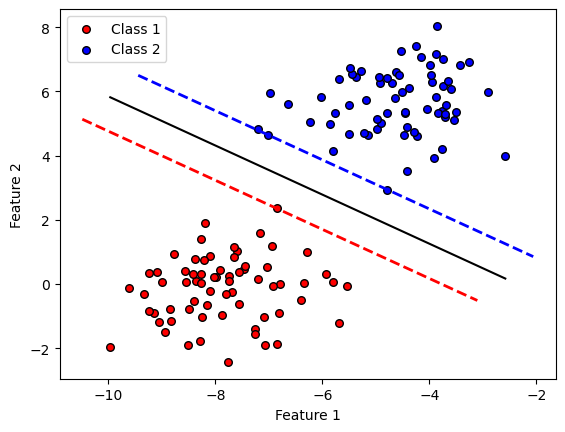
\includegraphics[width=\textwidth]{images/classicalsvm.png}
    \caption{SVM decision boundary and margin border, fitted on a 2 feature mock dataset of 200 instances.}
    \label{fig:classical svm mock}
\end{figure}

\subsubsection{Kernel SVM}
We now need to address the issue of dealing with a highly non-linearly separable dataset. Let's consider as an example another mock dataset, shown in Figure (\ref{fig:classical svm circles}). 
\begin{figure}[h!]
    \centering
    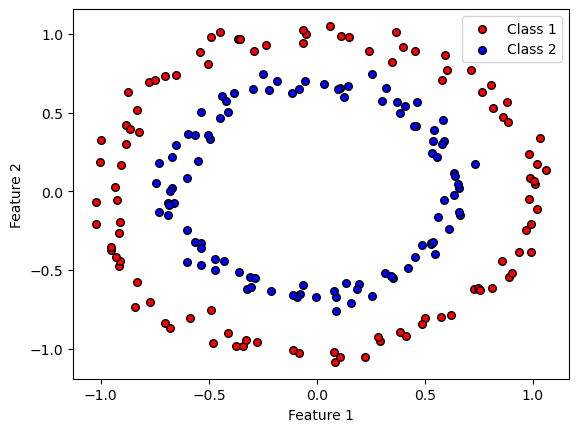
\includegraphics[width=\textwidth]{images/circles.png}
    \caption{Higly non-linear 2 feature mock dataset with 200 instances.}
    \label{fig:classical svm circles}
\end{figure}
It is clear that in this case we cannot use the SVM algorithm in its basic form, not even with a soft margin. We must introduce the idea of kernelization. 
Let's introduce a function, called feature map, which projects the data in a higher dimensional space. That means a function
\begin{equation}
    \phi:\mathbb{R}^d\rightarrow\mathbb{R}^D,
\end{equation}
with $D>d$. The codomain of the feature map is called feature space. If we choose a suitable feature map we can hope to obtain a linearly separable dataset in the feature space. The choice of the feature map is completely arbitrary, as long as it is a bijective function. Therefore, in principle, each time we are given a dataset we must choose an appropriate feature map for this strategy to work. For our example let's consider the feature map
$$    \phi:\mathbb{R}^2\rightarrow\mathbb{R}^3,$$
\begin{equation}
    \begin{pmatrix}
        x_0\\
        x_1
        \end{pmatrix} \mapsto  
        \begin{pmatrix}
        x_0^2 \\
        x_1^2\\
        \sqrt{2}x_0x_1
        \end{pmatrix} .
\end{equation}
The data of Figure (\ref{fig:classical svm circles}) after the application of the feature map $\phi$ are represented in Figure (\ref{fig:classical svm circle 3d}). 
\begin{figure}[h!]
    \centering
    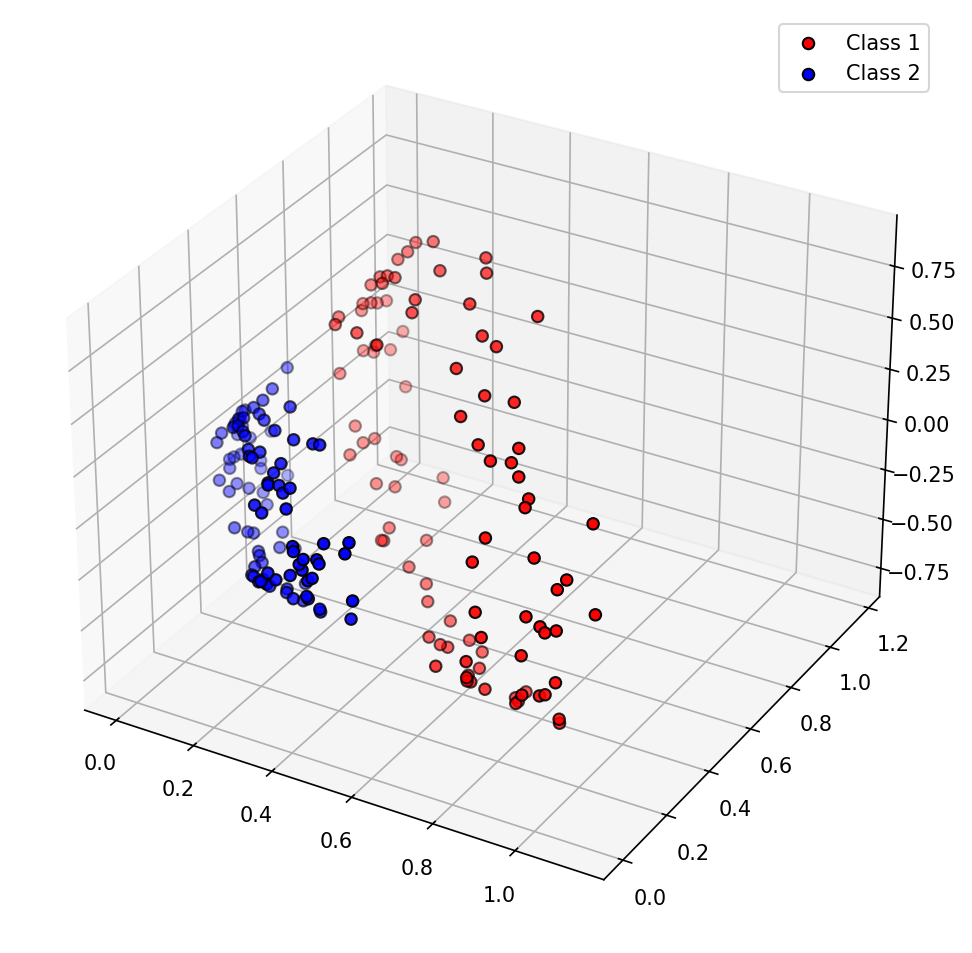
\includegraphics[width=\textwidth]{images/circles3d.png}
    \caption{Highly non-linear mock dataset in the feature space after the application of the feature map $\phi$. We observe now that the dataset is linearly separable.}
    \label{fig:classical svm circle 3d}
\end{figure}
The dataset is now linearly separable in the feature space, so the strategy worked. We can now apply the SVM algorithm in this space Consider the two central equations of the algorithm: equation (\ref{dual problem SVM}), which provides the expression to maximize in order to find the margin, and equation (\ref{decision boundary svm}), which gives the rule for predicting the class of a new instance. These two equations are now modified into 
\begin{equation}
    f(\alpha_0,\cdots,\alpha_{N-1})=\sum_{i=0}^{N-1} \alpha_i-\frac{1}{2}\sum_{i=0}^{N-1}\sum_{j=0}^{N-1}\alpha_i\alpha_jy_iy_j(\phi(\mathbf{x}_i,)\phi(\mathbf{x}_j)),
    \label{kernel max}
\end{equation}
\begin{equation}
    \textup{sign}\left[\sum_{i=0}^{N-1}\alpha_iy_i(\phi(\mathbf{\tilde{x}}), \phi(\mathbf{x}_i))+w_0\right].
    \label{kernel prodiction}
\end{equation}
A crucial observation is that in these two expressions only the scalar product of the feature map values appears. Therefore, we can conclude that the specific form of the feature map is not important, but rather the scalar product it produces. We can define the kernel $K$ as 
$$K:\mathbb{R}^d\times \mathbb{R}^d\rightarrow \mathbb{R},$$
\begin{equation}
    \mathbf{x}, \mathbf{y}\mapsto(\phi(\mathbf{x}), \phi(\mathbf{y})),
\end{equation}
 where $(\phi(\mathbf{x}), \phi(\mathbf{y}))=\phi(\mathbf{x})^T\cdot \phi(\mathbf{y})$ is the standard scalar product of $\mathbb{R}^D$. Eq. (\ref{kernel max}) and eq. (\ref{kernel prodiction}) now become 
 \begin{equation}
    f(\alpha_0,\cdots,\alpha_{N-1})=\sum_{i=0}^{N-1} \alpha_i-\frac{1}{2}\sum_{i=0}^{N-1}\sum_{j=0}^{N-1}\alpha_i\alpha_jy_iy_jK(\mathbf{x}_i,\mathbf{x}_j),
    \label{kernel max K}
\end{equation}
\begin{equation}
    \textup{sign}\left[\sum_{i=0}^{N-1}\alpha_iy_iK(\mathbf{\tilde{x}}, \mathbf{x}_i)+w_0\right].
    \label{kernel prodiction K}
\end{equation}
We see explicitly that the only quantity that matters is the kernel $K$. In our specific example the value of the kernel is 
\begin{equation}
    K(\mathbf{x}, \mathbf{y})= \begin{pmatrix}
        x_0^2 & x_1^2 & \sqrt{2}x_0x_1 \\
        \end{pmatrix}\cdot       \begin{pmatrix}
            y_0^2 \\
            y_1^2\\
            \sqrt{2}y_0y_1
            \end{pmatrix}=(\mathbf{x}^T\cdot\mathbf{y})^2.   
            \label{polykernel ex}   
\end{equation}
Therefore once we are given a dataset it is sufficient for us to choose an appropriate kernel, and forget about the feature map. Once the kernel has been chosen the SVM can be trained using eq. (\ref{kernel max K}), and we can use it to predict a new class using eq. (\ref{kernel prodiction K}). There are some properties that the kernel must satisfy:
\begin{itemize}
    \item The kernel must be symmetric, that is $$\forall\, \mathbf{x},\mathbf{y}\in \mathbb{R}^d,\,K(\mathbf{x},\mathbf{y})=K(\mathbf{y},\mathbf{x}).$$
    \item The kernel must be positive definite, that is $$\forall\, \mathbf{x},\mathbf{y}\in \mathbb{R}^d,\,K(\mathbf{x},\mathbf{y})\geq 0.$$
\end{itemize}
Common choices of kernels are
\begin{itemize}
    \item Linear kernel: $$K(\mathbf{x},\mathbf{y})=\mathbf{x}^T\cdot\mathbf{y}.$$ This goes back to the standard SVM we used in Figure (\ref{fig:classical svm mock}). It is suitable only for linearly separable (or close to, using soft margin) datasets.
    \item Polynomial kernel: $$K(\mathbf{x},\mathbf{y})=(\gamma\mathbf{x}^T\cdot\mathbf{y}+c)^\delta.$$ For $c=0$, $\gamma=1$ and $\delta=2$ we obtain the kernel of eq. (\ref{polykernel ex}). 
    \item Gaussian kernel: $$K(\mathbf{x},\mathbf{y})=\exp(-\gamma||\mathbf{x}-\mathbf{y}||).$$ This is also known as Radial Basis Function (RBF) kernel. 
    \item Sigmoid kernel: $$K(\mathbf{x},\mathbf{y})=\tanh(\mathbf{x}^T\cdot\mathbf{y}+c).$$
\end{itemize}
scikit learn offers an easy way to easily implement all these common kernels. For example the kernel in eq. (\ref{polykernel ex}) can be implemented as 
\begin{lstlisting}
    svm = SVC(kernel='poly', degree=2, gamma=1, coef0=0)
\end{lstlisting}\
One can also create a custom kernel, passing as an argument a callable function to be used to calculate the kernel. Fitting this SVC function to the non-linear dataset of Figure (\ref{fig:classical svm circles}) yields the result shown in Figure (\ref{fig:classical svm circle decision boundary}). 
\begin{figure}[h!]
    \centering
    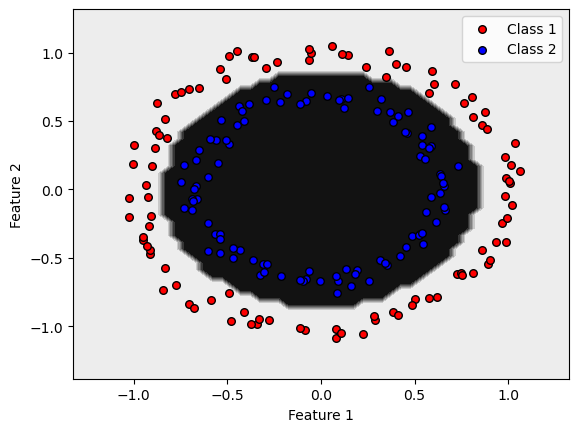
\includegraphics[width=\textwidth]{images/circlesclassicaldecisionboundary.png}
    \caption{Highly non-linear mock dataset decision boundary, fitted with a SVM using kernel of eq. (\ref{polykernel ex}). The white and black areas are the two predicted classes. We observe how, using the kernel, we obtained a non-linear decision boundary.}
    \label{fig:classical svm circle decision boundary}
\end{figure}
\newpage

\section{Quantum machine learning}
Introduction bla bla

\subsection{Quantum Support Vector Machine}
\subsubsection{Quantum feature map and Quantum Kernels}
The SVM algorithm faces some important limitations when the feature space becomes large, as estimating kernel functions becomes computationally intensive. Quantum computing could enhance the algorithm's performance by providing access to exponentially large Hilbert feature spaces. The idea is to construct a feature map which maps classical data into a quantum state which lives in an exponentially large Hilbert feature space. Therefore, in this context a feature map is a function 
\begin{equation}
    \phi: \mathbb{R}^d \rightarrow \mathcal{H},
\end{equation}
$$\mathbf{x}\mapsto \phi(\mathbf{x})\equiv |\phi(\mathbf{x})\rangle.$$
In the framework of quantum computing $\mathcal{H}$ is a $n$-qubit Hilbert space, that is a space of the form
\begin{equation}
    \mathcal{H}=\bigotimes_{i=0}^n \mathcal{H}_{qubit},
\end{equation}
where $\mathcal{H}_{qubit}$ is the Hilbert space of a single qubit. The dimension of $\mathcal{H}$ is $2^n$. The feature map will be implemented by the means of a parametrized quantum circuit. That means that it exists a unitary operator that depends on $d$ classical parameters $U(\mathbf{x})=U(x_0,\cdots, x_{d-1})$ such that 
\begin{equation}
    |\phi(\mathbf{x})\rangle=U(\mathbf{x})|0\rangle^{\otimes n}.
\end{equation}
This circuit is called quantum encoding circuit, because it encodes classical data into a quantum state. The classical data is passed to the circuit as a parameter. We will later make examples of frequently used encoding circuits. 
Once we have the feature map the kernel is constructed as 
\begin{equation}
    K(\mathbf{x}, \mathbf{y})=\left | \langle \phi(\mathbf{x})|\phi(\mathbf{y})\rangle \right |^2.
\end{equation}
Here $\langle\,\,, \,\rangle$ denotes the standard internal scalar product between vectors in $\mathcal{H}$. This definition clearly yields a kernel that satisfies the two kernel properties. How do we calculate the kernel in practice? Suppose we want to calculate the kernel $K(\mathbf{x}, \mathbf{y})$ and consider the following circuit. 

\begin{equation}
\Qcircuit @C=2em @R=2em {
   \lstick{|0\rangle} & \multigate{4}{U(\mathbf{x})} & \multigate{4}{U^\dagger(\mathbf{y})} & \meter\\
   \lstick{|0\rangle} & \ghost{U(\mathbf{x})}        & \ghost{U^\dagger(\mathbf{y})}        & \meter  \\
   \lstick{\vdots}    & \ghost{U(\mathbf{x})}        & \ghost{U^\dagger(\mathbf{y})}        & \vdots \\
   \lstick{|0\rangle} & \ghost{U(\mathbf{x})}        & \ghost{U^\dagger(\mathbf{y})}        & \meter  \\
   \lstick{|0\rangle} & \ghost{U(\mathbf{x})}        & \ghost{U^\dagger(\mathbf{y})}        & \meter  \\
} 
\label{circuit}
\end{equation}
\\
\noindent Suppose we run this circuit $R$ times, and we call $A$ the number of times that we measure the bit string $000\cdots 0$. We state that 
\begin{equation}
    \lim_{R\rightarrow +\infty}\frac{A}{R}=K(\mathbf{x}, \mathbf{y}).
    \label{frequency}
\end{equation}
The proof is straightforward. The LHS of eq. (\ref{frequency}) is the probability of measuring $000\cdots 0$, which according to quantum mechanics can be calculated as 
$$
    |^{\otimes n}\textrm{$\langle$}0|U(\mathbf{x})U^\dagger(\mathbf{y})|0\rangle^{\otimes n}|^2=|^{\otimes n}\textrm{$\langle$}0|U^\dagger(\mathbf{y})U(\mathbf{x})|0\rangle^{\otimes n}|^2=$$$$=|\langle \phi(\mathbf{y})|\phi(\mathbf{x})\rangle|^2=K(\mathbf{x}, \mathbf{y}).
$$
\hfill $\square$

\noindent Therefore, to evaluate the kernel, it suffices to construct the quantum circuit (\ref{circuit}) and measure the frequency with which the string $000\cdots 00$ occurs. We have to perform this operation for each pair of instances, and construct the matrix 
\begin{equation}
    K_{ij}=K(\mathbf{x}_i, \mathbf{x}_j).
\end{equation}
This kernel matrix is then plugged into eq. (\ref{kernel max K}) to train a classical SVM. 

\subsubsection{Quantum encoding circuits}
Let's now discuss some possible choices of quantum encoding circuits:
\begin{itemize}
    \item Basis encoding: this can be applied if the instances live in a finite dimensional space, whose dimension $2^n$, where $n$ is the number of qubits. If the dimension is smaller that $2^n$ we can still apply this encoding by using padding. The instances can be mapped into bit strings of length $n$ and the feature map corresponds to
    \begin{equation}
        \phi:\{0,1\}^n \rightarrow \mathcal{H},
    \end{equation}
    $$x=(x_0\cdots x_{n-1})\mapsto |x_0\rangle \otimes \cdots \otimes |x_{n-1}\rangle\equiv|x_0\cdots x_{n-1}\rangle=|x\rangle.$$ Here $|x\rangle$ is a state of the so called computational basis. For example the bit string $01001$ is mapped to the quantum state $$|0\rangle \otimes |1\rangle \otimes |0\rangle \otimes |0\rangle \otimes |1\rangle=|01001\rangle.$$ The kernel that originates from this feature map is 
    \begin{equation}
        K(x,y)=|\langle x|y\rangle|^2=|\delta_{x,y}|^2=\delta_{x,y}
    \end{equation}
    since vectors in the computational basis are orthogonal. 
    \item Amplitude encoding: this can be applied with instances that are normalized vector, that is vectors of the form 
    \begin{equation}
        \mathbf{x}=(x_0, \cdots, x_{d-1})^T\in \mathbb{R}^d,
    \end{equation}
    such that $$\sum_{i=0}^{d-1}x_i^2=1.$$
    In this case the encoding consists in sending
    \begin{equation}
        \mathbf{x}=(x_0, \cdots, x_{d-1})^T \mapsto |\phi(\mathbf{x})\rangle=\sum_{i=0}^{d-1}x_i|i\rangle,
    \end{equation}
    where $|i\rangle$ is the i-th vector of the computational basis. The fact that $\mathbf{x}$ is normalized ensures that the feature vector is normalized as well, and therefore represents a physical state. The kernel generated by this feature map is 
    \begin{equation}
        K(x,y)=\left|\sum_{i,j}x_iy_j\langle i|j\rangle\right|^2=\left|\sum_{i,j}x_iy_j\delta_{i,j}\right|^2=(\mathbf{x}^T \cdot \mathbf{y})^2.
    \end{equation}
    We went back to a polynomial kernel. 
    \item By creating more copies of the feature vector of amplitude encoding we can create higher order polynomial kernels. 
    \item Product encoding: in this case each feature of the input is encoded in the amplitudes of one separate qubit. For example, we can send
    \begin{equation}
        \mathbf{x}=(x_0, \cdots, x_{d-1})^T \mapsto  \begin{pmatrix}
            \cos x_0\\\sin x_0
           \end{pmatrix} \otimes \cdots \otimes \begin{pmatrix}
            \cos x_{d-1}\\\sin x_{d-1}
           \end{pmatrix},
    \end{equation}
    therefore the i-th qubit will be in the state 
    \begin{equation}
        \cos x_i|0\rangle +\sin x_i |1\rangle. 
    \end{equation}
    This generates the kernel 
    \begin{equation}
        K(x,y)=\prod_{i=0}^{d-1}\cos(x_i-y_i).
    \end{equation}
    \item ZZ feature map: The previously discussed encoding maps where quantum maps that in the end generated a kernel which is easy to calculate with classical tools, for example a polynomial kernel or a cosine kernel. It is important now to discuss quantum encoding circuits that creates a kernel which is not possible to write as an easy classical kernel, otherwise there is no advantage in using quantum computing for this task if the kernel could have been easily calculated with classical tools. The hope is that by using a purely quantum kernel we obtain better performance that by using a classical kernel. Since general quantum circuits are not expected to be classically simulable, there are many choices one can make. One example is generated by the following circuit 

    \[
        \Qcircuit @C=3em @R=2em {
        \lstick{|0\rangle} & \gate{H} & \multigate{4}{\,\,\,\,\mathcal{U}(\mathbf{x})\,\,\,\,} & \qw \\
        \lstick{|0\rangle} & \gate{H} & \ghost{\,\,\,\,\mathcal{U}(\mathbf{x})\,\,\,\,}        & \qw \\
        \lstick{\vdots}    & \vdots   & \ghost{\,\,\,\,\mathcal{U}(\mathbf{x})\,\,\,\,}                    & \vdots \\
        \lstick{|0\rangle} & \gate{H} & \ghost{\,\,\,\,\mathcal{U}(\mathbf{x})\,\,\,\,}        & \qw \\
        \lstick{|0\rangle} & \gate{H} & \ghost{\,\,\,\,\mathcal{U}(\mathbf{x})\,\,\,\,}        & \qw \\
        }
    \]  
    \\
    where $H$ is the standard Hadamard gate and 
    \begin{equation}
        \mathcal{U}(\mathbf{x})=\exp\left[i\sum_{S\subseteq [n]}\phi_S(\mathbf{x})\prod_{i\in S}Z_i\right].
        \label{ZZ}
    \end{equation}
    Here $[n]=\{0,\cdots, n-1\}$, $Z_i$ is the third Pauli matrix acting on the i-th qubit and $\phi_S(\mathbf{x})$ are arbitrary coefficients, which are the ones that actually encode the classical data. $S$ runs over all possible subsets of $[n]$, and can be thought as an index that describes connectivities between different qubits or data points. We have $2^n$ possible choices of the coefficients. It is convenient to choose them in a way such that only the terms with $|S|\leq d$ contribute, in order to obtain a circuit that can be easily implemented on a quantum computer. This is done by asking that
    \begin{equation}
        \phi_S=0\,\,\,\,\,\textup{if}\,\,\,\,\,|S|>d.
    \end{equation}
    Let's focus on a simple case where $n=d=2$. There are two default choices for the coefficients in this case. The first one is to set 
    \begin{equation}
        \phi_{\{i\}}(\mathbf{x})=x_i,
        \label{coeff Z}
    \end{equation}
    \begin{equation}
        \phi_{\{i,j\}}(\mathbf{x})=0.
    \end{equation}
    The feature map becomes 
    \begin{equation}
        {U}(\mathbf{x})=e^{ix_0Z_0}\,e^{ix_1Z_1}H^{\otimes n}.
    \end{equation}
    This is called Z feature map. The circuit decomposed in elementary quantum gates is shown in Figure \ref{fig:Z}. 
    \begin{figure}[h!]
        \centering
        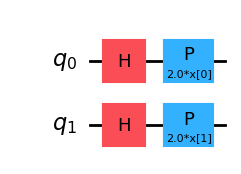
\includegraphics[height=100px]{images/Z.png}
        \caption{Z feature map, with 2 qubits and 2 features, decomposed in terms of elementary gates. The gate $P$ is defined as $P(\phi) = (1,0; 0, e^{i\phi})$. We observe how the circuit is parametrized by the coefficients of eq. (\ref{coeff Z}).}
        \label{fig:Z}
    \end{figure}
    The other possible choice is  
    \begin{equation}
        \phi_{\{i\}}(\mathbf{x})=x_i,
        \label{coeff ZZ1}
    \end{equation}
    \begin{equation}
        \phi_{\{i,j\}}(\mathbf{x})=(\pi-x_i)(\pi-x_j).
        \label{coeff ZZ2}
    \end{equation}
    In this case the feature maps becomes 
    \begin{equation}
        {U}(\mathbf{x})=e^{i(\pi-x_0)(\pi-x_1)Z_0Z_1}\,e^{ix_0Z_0}\,e^{ix_1Z_1}H^{\otimes n}.
    \end{equation}
    This is called ZZ feature map, and it is an encoding circuit thought to be hard to simulate classically. It is shown in Figure \ref{fig:ZZ}. 
    \begin{figure}[h!]
        \centering
        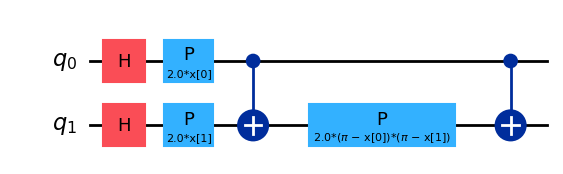
\includegraphics[height=100px]{images/ZZ.png}
        \caption{ZZ feature map, with 2 qubits and 2 features, decomposed in terms of elementary gates. The gate $P$ is defined as $P(\phi) = (1,0; 0, e^{i\phi})$. We observe how the circuit is parametrized by the coefficients of eq. (\ref{coeff ZZ1}) and (\ref{coeff ZZ2}).}
        \label{fig:ZZ}
    \end{figure}
    We will see how it behaves later on. Those two are standard choices, but there are many more circuits that can be built starting from the general structure of eq. (\ref{ZZ}), especially if we consider a greater number of qubits, and so we allow connectivities of three and more qubits. 
    \item Pauli feature map: Eq. (\ref{ZZ}) can be generalised to include not only Z gates, but all of the Pauli gates. We can have
    \begin{equation}
        \mathcal{U}(\mathbf{x})=\exp\left[i\sum_{S\subseteq [n]}\phi_S(\mathbf{x})\prod_{i\in S}P_i\right],
        \label{pauli}
    \end{equation}
    where $P\in\{1,X,Y,Z\}$. This allows us to generate not only interaction of the ZZ type, but also for example YY type or ZY type. An example with Y and ZY interactions is shown in Figure \ref{pauli}.
    \begin{figure}[h!]
        \centering
        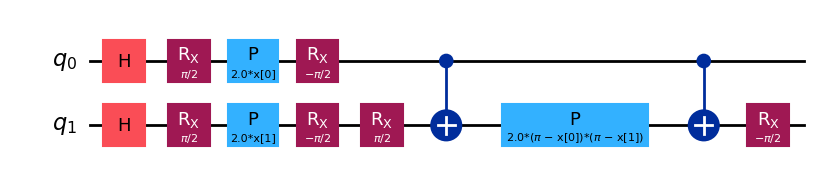
\includegraphics[width=\textwidth]{images/pauli.png}
        \caption{Pauli feature map, with 2 qubits and 2 features, decomposed in term of elementary gates, constructed with Y and YZ interactions.}
        \label{fig:Pauli}
    \end{figure}
    \item In general any parametrized quantum circuit can be used to encode classical data and create a quantum kernel. We will later use generic circuits and study what sort of datasets they separate.
\end{itemize}

\subsubsection{QSVM algorithm and Qiskit implementation}
To sum things up the step of the Quantum Support Vector Machine (QSVM) algorithm are
\begin{itemize}
    \item Prepare the classical data into two vectors $X$ and $y$, where $$X_i=\mathbf{x}_i \in \mathbb{R}^d,\, \,\,\,i=0,\cdots , N-1,$$ is the i-th $d$-dimensional instance, and $$y_i\in \{-1,1\},$$ indicates the class that this instance belongs to.  
    \item Choose a parametrized quantum circuit $U(\mathbf{x})$. The circuit accepts $d$ parameters, which are the features of the instance we are considering. One can choose a standard circuit like the ZZ feature map, or can create a custom circuit. We will extensively revisit the point of choosing the circuit later on.
    \item For each pair of instances $\mathbf{x}_i$, $\mathbf{x}_j$ we must evaluate the kernel matrix $$K_{ij}=K(\mathbf{x}_i,\mathbf{x}_j).$$ This is an $N\times N$ matrix, so for each pair we have build $U(\mathbf{x}_i)$ and $U^\dagger(\mathbf{x}_j)$, in order to construct the circuit     
    \begin{equation}
        \Qcircuit @C=2em @R=2em {
           \lstick{|0\rangle} & \multigate{4}{U(\mathbf{x}_i)} & \multigate{4}{U^\dagger(\mathbf{\mathbf{x}_j})} & \meter\\
           \lstick{|0\rangle} & \ghost{U(\mathbf{x}_i)}        & \ghost{U^\dagger(\mathbf{\mathbf{x}_j})}        & \meter  \\
           \lstick{\vdots}    & \ghost{U(\mathbf{x}_i)}        & \ghost{U^\dagger(\mathbf{\mathbf{x}_j})}        & \vdots \\
           \lstick{|0\rangle} & \ghost{U(\mathbf{x}_i)}        & \ghost{U^\dagger(\mathbf{\mathbf{x}_j})}        & \meter  \\
           \lstick{|0\rangle} & \ghost{U(\mathbf{x}_i)}        & \ghost{U^\dagger(\mathbf{\mathbf{x}_j})}        & \meter  \\
        } 
        \label{circuit item }
    \end{equation}
    and evaluate the matrix element 
    \begin{equation}
        K_{ij}=|^{\otimes n}\textrm{$\langle$}0|U(\mathbf{x}_iU^\dagger(\mathbf{x}_j)|0\rangle^{\otimes n}|^2.        
    \end{equation}
    As we saw this can be done, up to an error $R^{-1/2}$, by running the circuit (\ref{circuit item }) $R$ times and counting the number of times that we measure the string $000\cdots 0$.
    \item Once we have the kernel matrix we use classical optimization to maximize
    \begin{equation}
        f(\alpha_0,\cdots,\alpha_{N-1})=\sum_{i=0}^{N-1} \alpha_i-\frac{1}{2}\sum_{i=0}^{N-1}\sum_{j=0}^{N-1}\alpha_i\alpha_jy_iy_jK_{ij}.
    \end{equation}
    Once we found the optimal $\alpha$ we have constructed the decision boundary.
    \item Given a new instance $\tilde{\mathbf{x}}$ we can, in the same way, calculate the kernel matrix element $$\tilde{K}_i=K(\mathbf{x}_i, \tilde{\mathbf{x}}),$$ and predict the class of $\tilde{\mathbf{x}}$ by applying \begin{equation}
        \tilde{y}=\textup{sign}\left[\sum_{i=0}^{N-1}\alpha_iy_i\tilde{K}_i+w_0\right].
    \end{equation}
\end{itemize}

Schematically we have 

\begin{algorithm}[H]
    \caption{Quantum Support Vector Machine (QSVM)}
    \begin{algorithmic}[1]
        \State \textbf{Input:} Data $\{(\mathbf{x}_i, y_i)\}_{i=0,\cdots,N-1}$, Quantum circuit $U(\mathbf{x})$
        \State \textbf{Parameters:} Measurement shots $R$
        
        \For{$i = 0 \textbf{ to } N-1$}
            \For{$j = 0 \textbf{ to } N-1$}
                \State \textbf{Prepare} $U(\mathbf{x}_i)$ and $U^\dagger(\mathbf{x}_j)$
                \State \textbf{Run} circuit $U(\mathbf{x}_i)U^\dagger(\mathbf{x}_j)$ $R$ times  
                \State \textbf{Measure} the frequency $f$ of $00\cdots 0$ 
                \State \textbf{Set} $f=K_{ij}$ 
            \EndFor
        \EndFor
        
        \State \textbf{Optimize} $\alpha$ to maximize
        \begin{equation*}
            f(\alpha) = \sum_{i=0}^{N-1} \alpha_i - \frac{1}{2} \sum_{i=0}^{N-1} \sum_{j=0}^{N-1} \alpha_i \alpha_j y_i y_j K_{ij}
        \end{equation*}
    
        \For{each new instance $\tilde{\mathbf{x}}$}
            \State \textbf{Compute} $\tilde{K}_i = K(\mathbf{x}_i, \tilde{\mathbf{x}})$
            \State \textbf{Predict} $\tilde{y} = \textup{sign}\left(\sum_{i=0}^{N-1} \alpha_i y_i \tilde{K}_i + w_0\right)$
        \EndFor
        
    \end{algorithmic}
    \end{algorithm}

This algorithm can be implemented in practice exploiting Qiskit to perform the circuit simulation and calculate the kernel, and subsequently using scikit-learn to perform the classical optimization once the kernel has been calculated. We can make an example, separating a mock dataset like in Figure \ref{fig:classical svm mock}, with a Pauli feature map. 

\begin{lstlisting}
    #create mock dataset
    X,y=make_blobs(n_samples=200) 
    #since the kernel involves rotation it is better to bring the data between 0 and pi
    X=MinMaxScaler(feature_range=(0,np.pi)).fit_transform(X) 
    #create quantum kernel
    kernel=FidelityQuantumKernel(feature_map=ZFeatureMap()) 
    #pass the kernel as a callable function 
    svm=SVC(kernel=kernel.evaluate) 
    #fit the svm
    svm.fit(X, y) 
\end{lstlisting}

The result of the fit is shown in Figure \ref{fig:qsvm}.
\begin{figure}[h!]
    \centering
    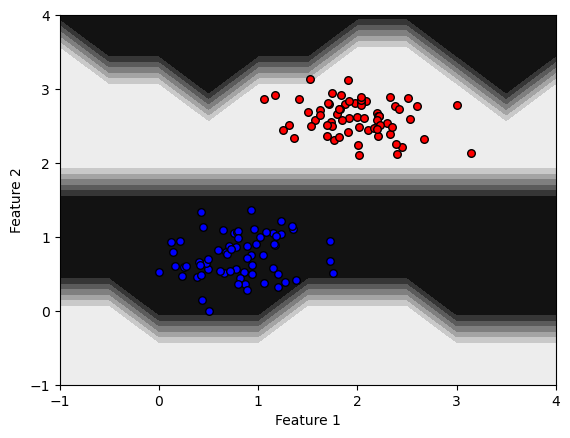
\includegraphics[width=\textwidth]{images/qsvm.png}
    \caption{QSVM decision boundary with ZFeatureMap, fitted on a 2 feature mock dataset of 200 instances.}
    \label{fig:qsvm}
\end{figure}

\subsubsection{QSVM potential}
In order to study the potential of the QSVM algorithm we could try and observe the form of the decision boundary of an artificial dataset which is easily separable by a QSVM. If the decision boundary is "classically looking", that is similar to the one we observed when we studied the linear or polynomial kernel, then it would look like the QSVM algorithm may not provide advantage over the classical SVM. We hope instead to find a complex looking decision boundary, which is not separable by classical kernels. 

We use ZZFeatureMap, with $n=d=2$. Furthermore, we choose $f=Z_1Z_2$ and $V\in\textup{SU}(4)$. We assign $m(\mathbf{x})=+1$ when 
\begin{equation}
    \langle \phi(\mathbf{x}) |V^\dagger f V|\phi(\mathbf{x})\rangle >\Delta,
\end{equation} 
and $m(\mathbf{x})=-1$ when 
\begin{equation}
    \langle \phi(\mathbf{x}) |V^\dagger f V|\phi(\mathbf{x})\rangle <\Delta.
\end{equation} 
$\Delta$ controls how big is the gap between of the two classes. We show this dataset in Figure \ref{fig:adhoc}.
\begin{figure}[h!]
    \centering
    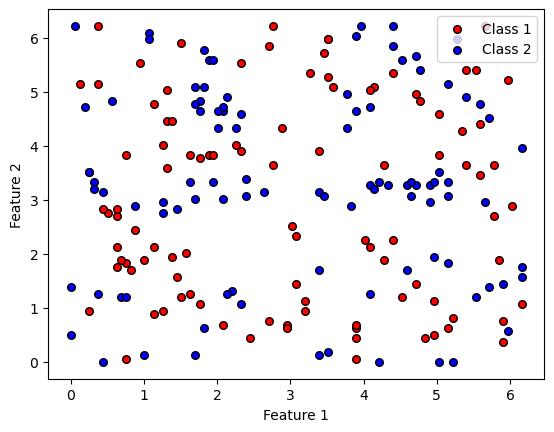
\includegraphics[width=\textwidth]{images/adhoc.png}
    \caption{Artificial ad hoc dataset, generated with $\Delta=0.3$. This dataset, by construction, is easily separable by ZZFeatureMap.}
    \label{fig:adhoc}
\end{figure}
We observe how the dataset of Figure \ref{fig:adhoc} shows a very complicated pattern. Classical methods cannot hope to separate these two classes. In fact, if we divide the dataset into a training set and a test set, and apply the classical SVM algorithm, for example with the RBF kernel, we obtain an accuracy on the test set of 0.51, which is essentially like assigning the classes with a random coin toss. The result of the classical fit is shown in Figure \ref{fig:adhocrbf}, in which we observe how the correct decision boundary has not been found. 
\begin{figure}[h!]
    \centering
    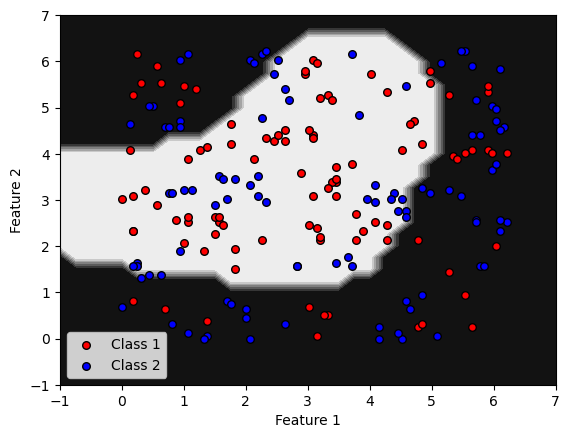
\includegraphics[width=\textwidth]{images/adhocrbf.png}
    \caption{Result of the classical fit with RBF kernel on the artificial dataset. We observe how the SVM could not find the correct separation between the classes. }
    \label{fig:adhocrbf}
\end{figure}
In Figure \ref{fig:adhoczz} is shown instead the result of the fit with the QSVM with ZZFeatureMap, which yields an accuracy on the test set of 1.0, and a nice looking decision boundary. 
\begin{figure}[h!]
    \centering
    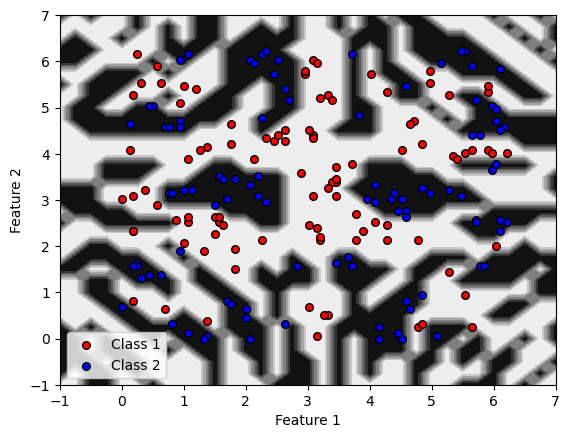
\includegraphics[width=\textwidth]{images/adhoczz.png}
    \caption{Result of the quantum fit on the artificial dataset, with ZZFeatureMap. We observe how the QSVM found the correct separation between the classes.}
    \label{fig:adhoczz}
\end{figure}

Finding a dataset which is separable by quantum methods and not by classical methods leads us into thinking that the QSVM algorithm might outperform the SVM algorithm on datasets with complex patterns, which is the result we hoped to find. 

\subsubsection{Issues of QSVM}

In a QSVM algorithm the only choice the user has to make is the choice of the feature map, that is the choice of the quantum encoding circuit. It is easy to convince ourselves that this choice is crucial, and determines if the algorithm will be successful or not. In the classical case we also have to choose a kernel, but we found that this choice is much less delicate that in the quantum case. In fact, for example, the RBF kernel works very well for most applications. In the quantum case instead, we observed that the choice of the feature map is very tricky. If the wrong feature map is chosen, the QSVM performs very poorly even on very simple datasets, as we will now illustrate with some examples. Let's consider the dataset shown in Figure , which is simple enough to be expected to be separated without too many difficulties. The RBF kernel separates this dataset very well. Let's try to apply some of the quantum kernels we discussed in the previous sections. 


We see how the results of the fits are not satisfying. The accuracy may not be too low in some cases, but the form of the decision boundary tells us that the algorithm did not find the correct pattern for the data. With more complex dataset the algorithm may fail completely, like shown in Figure .

It is clear at this point that the choice of the quantum encoding map is a very delicate part of the algorithm, and cannot be taken lightly. Choosing the feature map by trying the most common ones, as one may do with classical SVM, is not a safe method, as for a lot of datasets, even simple ones, the QSVM may fail. We need a more systematic way to choose the encoding. We will discuss those methods in the next sections.

\subsection{Quantum kernel alignment}

In the previous sections we discussed how 



\end{document}